\documentclass[twoside]{article}\usepackage[]{graphicx}\usepackage[]{color}
% maxwidth is the original width if it is less than linewidth
% otherwise use linewidth (to make sure the graphics do not exceed the margin)
\makeatletter
\def\maxwidth{ %
  \ifdim\Gin@nat@width>\linewidth
    \linewidth
  \else
    \Gin@nat@width
  \fi
}
\makeatother

\definecolor{fgcolor}{rgb}{0.345, 0.345, 0.345}
\newcommand{\hlnum}[1]{\textcolor[rgb]{0.686,0.059,0.569}{#1}}%
\newcommand{\hlstr}[1]{\textcolor[rgb]{0.192,0.494,0.8}{#1}}%
\newcommand{\hlcom}[1]{\textcolor[rgb]{0.678,0.584,0.686}{\textit{#1}}}%
\newcommand{\hlopt}[1]{\textcolor[rgb]{0,0,0}{#1}}%
\newcommand{\hlstd}[1]{\textcolor[rgb]{0.345,0.345,0.345}{#1}}%
\newcommand{\hlkwa}[1]{\textcolor[rgb]{0.161,0.373,0.58}{\textbf{#1}}}%
\newcommand{\hlkwb}[1]{\textcolor[rgb]{0.69,0.353,0.396}{#1}}%
\newcommand{\hlkwc}[1]{\textcolor[rgb]{0.333,0.667,0.333}{#1}}%
\newcommand{\hlkwd}[1]{\textcolor[rgb]{0.737,0.353,0.396}{\textbf{#1}}}%
\let\hlipl\hlkwb

\usepackage{framed}
\makeatletter
\newenvironment{kframe}{%
 \def\at@end@of@kframe{}%
 \ifinner\ifhmode%
  \def\at@end@of@kframe{\end{minipage}}%
  \begin{minipage}{\columnwidth}%
 \fi\fi%
 \def\FrameCommand##1{\hskip\@totalleftmargin \hskip-\fboxsep
 \colorbox{shadecolor}{##1}\hskip-\fboxsep
     % There is no \\@totalrightmargin, so:
     \hskip-\linewidth \hskip-\@totalleftmargin \hskip\columnwidth}%
 \MakeFramed {\advance\hsize-\width
   \@totalleftmargin\z@ \linewidth\hsize
   \@setminipage}}%
 {\par\unskip\endMakeFramed%
 \at@end@of@kframe}
\makeatother

\definecolor{shadecolor}{rgb}{.97, .97, .97}
\definecolor{messagecolor}{rgb}{0, 0, 0}
\definecolor{warningcolor}{rgb}{1, 0, 1}
\definecolor{errorcolor}{rgb}{1, 0, 0}
\newenvironment{knitrout}{}{} % an empty environment to be redefined in TeX

\usepackage{alltt}
\usepackage[utf8]{inputenc}
\usepackage[czech]{babel}
\usepackage{fancyhdr}
\usepackage[paper=a4paper, nomarginpar, foot=1.5cm, top=2.5cm, bottom=2.5cm, left=2.5cm, right=2.5cm]{geometry}
\usepackage{siunitx}

\pagestyle{fancy}
\fancyhead{} % clear all header fields
\fancyhead[RO,LE]{Marek Földi}
\fancyhead[RE,LO]{Úkol 1}
\fancyfoot{} % clear all footer fields
\fancyfoot[LE,RO]{\thepage}

\addto\captionsczech{\renewcommand{\figurename}{Graf. č.}}
\IfFileExists{upquote.sty}{\usepackage{upquote}}{}
\begin{document}




\subsection*{Příklad 1:}
\begin{knitrout}
\definecolor{shadecolor}{rgb}{0.969, 0.969, 0.969}\color{fgcolor}\begin{kframe}
\begin{alltt}
\hlkwd{mean}\hlstd{(zapesti.leve)}
\end{alltt}
\begin{verbatim}
## [1] 157.7857
\end{verbatim}
\begin{alltt}
\hlkwd{median}\hlstd{(zapesti.leve)}
\end{alltt}
\begin{verbatim}
## [1] 155
\end{verbatim}
\begin{alltt}
\hlkwd{quantile}\hlstd{(zapesti.leve)}
\end{alltt}
\begin{verbatim}
##   0%  25%  50%  75% 100% 
##  130  150  155  165  201
\end{verbatim}
\begin{alltt}
\hlkwd{sd}\hlstd{(zapesti.leve)}
\end{alltt}
\begin{verbatim}
## [1] 12.38634
\end{verbatim}
\begin{alltt}
\hlkwd{mean}\hlstd{(bota)}
\end{alltt}
\begin{verbatim}
## [1] 40.04643
\end{verbatim}
\begin{alltt}
\hlkwd{median}\hlstd{(bota)}
\end{alltt}
\begin{verbatim}
## [1] 39
\end{verbatim}
\begin{alltt}
\hlkwd{quantile}\hlstd{(bota)}
\end{alltt}
\begin{verbatim}
##   0%  25%  50%  75% 100% 
##   36   38   39   42   48
\end{verbatim}
\begin{alltt}
\hlkwd{sd}\hlstd{(bota)}
\end{alltt}
\begin{verbatim}
## [1] 2.71281
\end{verbatim}
\end{kframe}
\end{knitrout}

Průměr šířky levého zápěstí je 157,79~\si{\milli\metre}, medián je 155~\si{\milli\metre}, první kvartily 150~\si{\milli\metre}, třetí kvartil 165~\si{\milli\metre} a směrodatná odchylka je 12,39. Průměr velikosti bot je 40,05, medián je 39, první kvartil 38, třetí kvartil 42 a směrodatná odchylka je 2,71.

\subsection*{Příklad 2:}
\begin{knitrout}
\definecolor{shadecolor}{rgb}{0.969, 0.969, 0.969}\color{fgcolor}\begin{kframe}
\begin{alltt}
\hlkwd{cor}\hlstd{(zapesti.leve, bota)}
\end{alltt}
\begin{verbatim}
## [1] 0.6784696
\end{verbatim}
\end{kframe}
\end{knitrout}

Z~korelačního koeficientu můžeme říct, že hodnoty na sobě pozitivně závisí a je u~nich středně těsná závislost. Závislost můžeme také pozorovat na grafu č. \ref{fig:plot2}.
\begin{knitrout}
\definecolor{shadecolor}{rgb}{0.969, 0.969, 0.969}\color{fgcolor}\begin{kframe}
\begin{alltt}
\hlkwd{scatterplot}\hlstd{(zapesti.leve}\hlopt{~}\hlstd{bota,} \hlkwc{regLine}\hlstd{=}\hlnum{TRUE}\hlstd{,} \hlkwc{smooth}\hlstd{=}\hlnum{FALSE}\hlstd{,} \hlkwc{boxplots}\hlstd{=}\hlnum{FALSE}\hlstd{)}
\end{alltt}
\end{kframe}\begin{figure}[h]
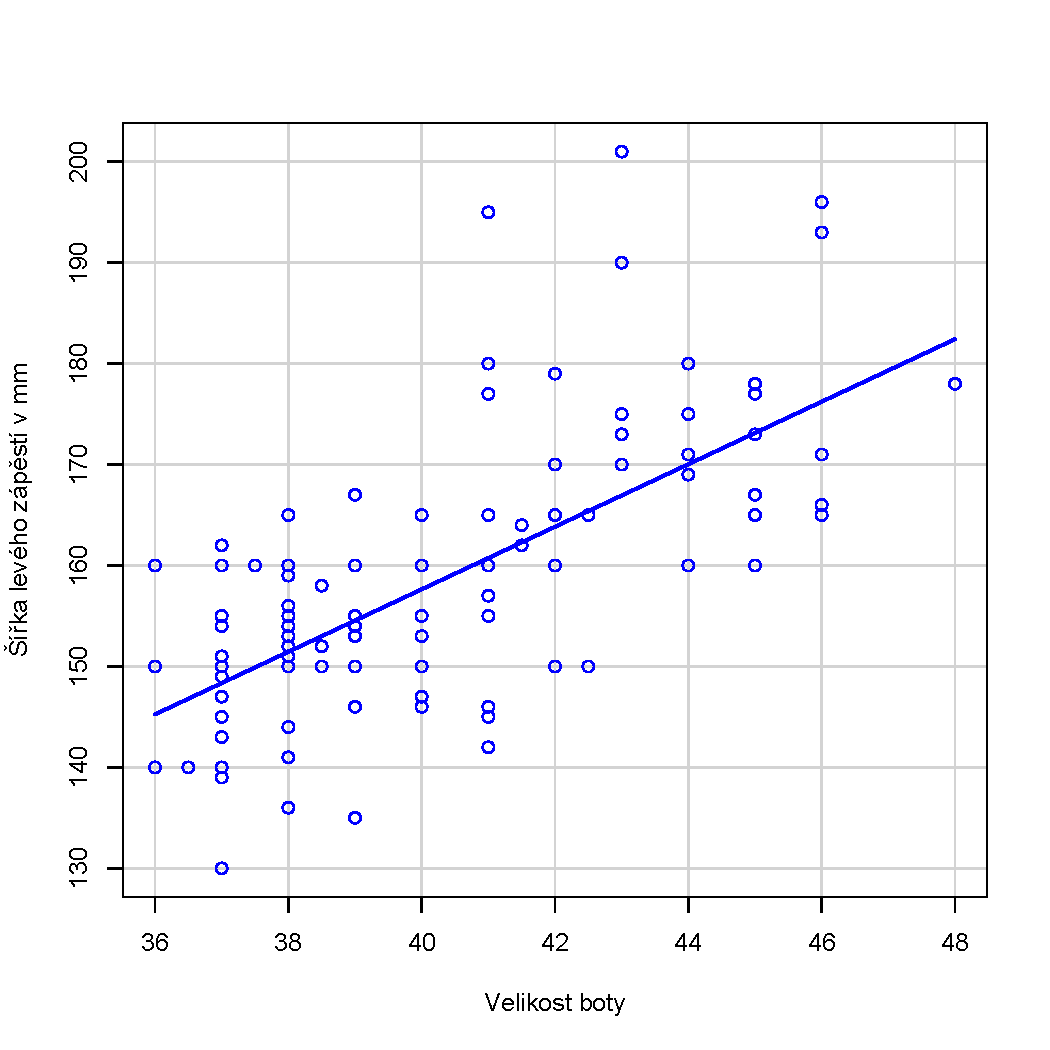
\includegraphics[width=\maxwidth]{figure/plot2-1} \caption[Závislost mezi velikostí bot a velikosti zápěstí]{Závislost mezi velikostí bot a velikosti zápěstí}\label{fig:plot2}
\end{figure}


\end{knitrout}


\newpage
\subsection*{Příklad 3:}
\begin{knitrout}
\definecolor{shadecolor}{rgb}{0.969, 0.969, 0.969}\color{fgcolor}\begin{kframe}
\begin{alltt}
\hlkwd{tapply}\hlstd{(zapesti.leve, pohlavi, summary)}
\end{alltt}
\begin{verbatim}
## $F
##    Min. 1st Qu.  Median    Mean 3rd Qu.    Max. 
##   130.0   150.0   153.0   152.9   160.0   179.0 
## 
## $M
##    Min. 1st Qu.  Median    Mean 3rd Qu.    Max. 
##   150.0   165.0   170.0   171.4   177.0   201.0
\end{verbatim}
\end{kframe}
\end{knitrout}
Průměry velikosti zápěstí se mezi pohlavími liší. U~mužů je větší než u~žen. Graficky můžeme znázornit pomocí \emph{plot of means} viz. graf č. \ref{fig:plot3}.

\begin{knitrout}
\definecolor{shadecolor}{rgb}{0.969, 0.969, 0.969}\color{fgcolor}\begin{kframe}
\begin{alltt}
\hlkwd{plotMeans}\hlstd{(zapesti.leve, pohlavi,} \hlkwc{error.bars}\hlstd{=}\hlstr{"se"}\hlstd{,} \hlkwc{main}\hlstd{=}\hlstr{""}\hlstd{,} \hlkwc{connect}\hlstd{=}\hlnum{FALSE}\hlstd{)}
\end{alltt}
\end{kframe}\begin{figure}[h]
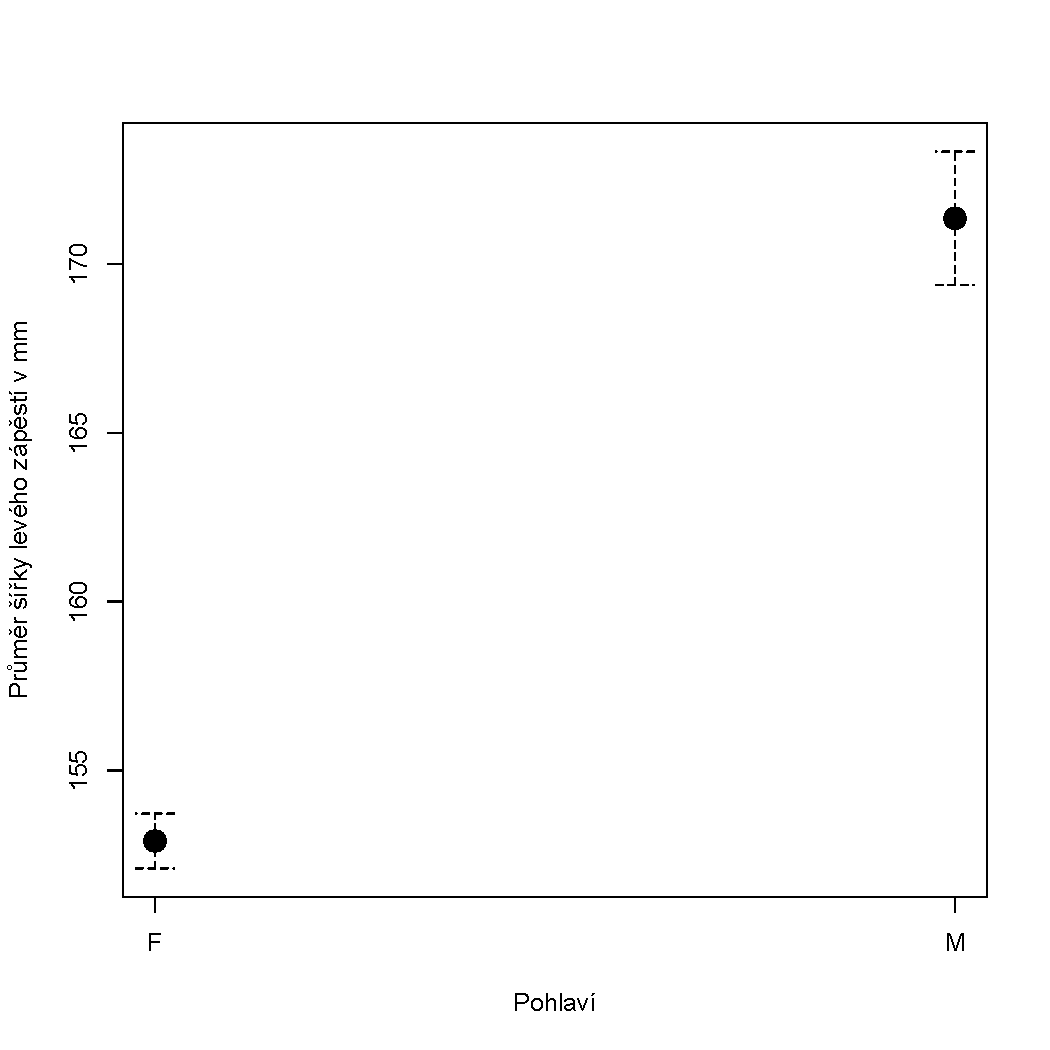
\includegraphics[width=\maxwidth]{figure/plot3-1} \caption[Závislost mezi velikostí bot a velikosti zápěstí]{Závislost mezi velikostí bot a velikosti zápěstí}\label{fig:plot3}
\end{figure}


\end{knitrout}


\newpage
\end{document}
